\documentclass[11pt]{article}

% ---------- Basic packages ----------
\usepackage[T1]{fontenc}
\usepackage{lmodern}
\usepackage{microtype}
\usepackage[margin=1in,headheight=15pt]{geometry}
\usepackage{graphicx}
\usepackage{amsmath,amssymb,amsthm}
\usepackage{mathtools}
\usepackage{tikz}
\usetikzlibrary{arrows.meta}
\usepackage{pgfplots}
\usepgfplotslibrary{groupplots}
\pgfplotsset{compat=1.18}
\usepackage[most]{tcolorbox}
\usepackage{xcolor}
\usepackage{fancyhdr}
\usepackage{titlesec}
\usepackage{enumitem}
\usepackage[hidelinks]{hyperref}
\usepackage{cleveref}
\usepackage{float}
\setlength{\parindent}{0pt}
\setlength{\parskip}{6pt}

% ---------- Document information ----------
\author{Ellie Su}
\hypersetup{
    pdftitle={Mass Conservation and Differential Formulation},
    pdfauthor={Ellie Su}
}

% ---------- Colors ----------
\definecolor{deepblue}{HTML}{315A78}
\definecolor{softblue}{HTML}{EFF7FC}
\definecolor{purple}{HTML}{745A8D}
\definecolor{softpurple}{HTML}{F5F0FA}
\definecolor{green}{HTML}{527A63}
\definecolor{softgreen}{HTML}{EFF8F3}
\definecolor{pink}{HTML}{A76578}
\definecolor{softpink}{HTML}{FFF2F5}
\definecolor{gold}{HTML}{A78032}
\definecolor{softyellow}{HTML}{FFF9E8}
\definecolor{softgray}{HTML}{F7F7F7}
\definecolor{grayborder}{HTML}{888888}

% ---------- Theorem heading styles (no parentheses around titles) ----------
\newtheoremstyle{plaincolon}
    {6pt}{6pt}{\itshape}{}{\bfseries}{.}{0.5em}
    {\thmname{#1}\thmnumber{ #2}\thmnote{: #3}}
\newtheoremstyle{definitioncolon}
    {6pt}{6pt}{}{}{\bfseries}{.}{0.5em}
    {\thmname{#1}\thmnumber{ #2}\thmnote{: #3}}
\newtheoremstyle{remarkcolon}
    {6pt}{6pt}{}{}{\itshape}{.}{0.5em}
    {\thmname{#1}\thmnumber{ #2}\thmnote{: #3}}

% ---------- Theorem environments ----------
\theoremstyle{plaincolon}
\newtheorem{theorem}{Theorem}[section]
\newtheorem{lemma}[theorem]{Lemma}
\newtheorem{proposition}[theorem]{Proposition}
\newtheorem{corollary}[theorem]{Corollary}
\theoremstyle{definitioncolon}
\newtheorem{definition}[theorem]{Definition}
\newtheorem{example}[theorem]{Example}
\newtheorem{problem}{Problem} % independent numbering: 1, ..., 10
\newtheorem{salvage}[theorem]{Salvage}
\theoremstyle{remarkcolon}
\newtheorem{remark}[theorem]{Remark}

% ---------- Proof-style environments ----------
\newenvironment{disproof}{\begin{proof}[Disproof]}{\end{proof}}
\newenvironment{solution}{\begin{proof}[Solution]}{\end{proof}}

% ---------- General box style ----------
\tcbset{
    mathematicalbox/.style={
        enhanced,
        breakable,
        boxrule=0.8pt,
        arc=2.5mm,
        left=10pt,
        right=10pt,
        top=8pt,
        bottom=8pt,
        before skip=10pt,
        after skip=10pt,
        fonttitle=\bfseries
    }
}

% ---------- General-purpose box ----------
\newtcolorbox{mathbox}[1][]{
    mathematicalbox,
    colback=white,
    colframe=deepblue,
    coltitle=deepblue,
    borderline west={3pt}{0pt}{deepblue},
    #1
}

% ---------- Theorem and proposition boxes ----------
\tcolorboxenvironment{theorem}{
    mathematicalbox,
    colback=softblue,
    colframe=deepblue,
    borderline west={3pt}{0pt}{deepblue}
}
\tcolorboxenvironment{proposition}{
    mathematicalbox,
    colback=softblue,
    colframe=deepblue,
    borderline west={3pt}{0pt}{deepblue}
}
% ---------- Lemma boxes ----------
\tcolorboxenvironment{lemma}{
    mathematicalbox,
    colback=softpurple,
    colframe=purple,
    borderline west={3pt}{0pt}{purple}
}
% ---------- Corollary boxes ----------
\tcolorboxenvironment{corollary}{
    mathematicalbox,
    colback=softgreen,
    colframe=green,
    borderline west={3pt}{0pt}{green}
}
% ---------- Definition boxes ----------
\tcolorboxenvironment{definition}{
    mathematicalbox,
    colback=softpink,
    colframe=pink,
    borderline west={3pt}{0pt}{pink}
}
% ---------- Example boxes ----------
\tcolorboxenvironment{example}{
    mathematicalbox,
    colback=softgreen,
    colframe=green,
    borderline west={3pt}{0pt}{green}
}
% ---------- Problem boxes ----------
\tcolorboxenvironment{problem}{
    mathematicalbox,
    colback=softyellow,
    colframe=gold,
    borderline west={3pt}{0pt}{gold}
}
% ---------- Salvage boxes ----------
\tcolorboxenvironment{salvage}{
    mathematicalbox,
    colback=softpurple,
    colframe=purple,
    borderline west={3pt}{0pt}{purple}
}
% ---------- Remark boxes ----------
\tcolorboxenvironment{remark}{
    enhanced,
    breakable,
    colback=white,
    colframe=grayborder,
    boxrule=0.7pt,
    arc=2.5mm,
    left=10pt,
    right=10pt,
    top=8pt,
    bottom=8pt,
    before skip=10pt,
    after skip=10pt,
    frame style={dash pattern=on 3pt off 2pt}
}
% ---------- Proof, disproof, and solution boxes ----------
\tcolorboxenvironment{proof}{
    enhanced,
    breakable,
    colback=softgray,
    colframe=grayborder,
    boxrule=0.5pt,
    arc=2mm,
    left=10pt,
    right=10pt,
    top=8pt,
    bottom=8pt,
    before skip=8pt,
    after skip=10pt,
    borderline west={2pt}{0pt}{grayborder}
}

% ---------- Section headings ----------
\titleformat{\section}
    {\Large\bfseries\color{deepblue}}
    {\thesection.}{0.5em}{}
    [\vspace{2pt}\color{deepblue}\titlerule]
\titleformat{name=\section,numberless}
    {\Large\bfseries\color{deepblue}}
    {}{0pt}{}
    [\vspace{2pt}\color{deepblue}\titlerule]
\titleformat{\subsection}
    {\large\bfseries\color{purple}}
    {\thesubsection.}{0.5em}{}
\titleformat{name=\subsection,numberless}
    {\large\bfseries\color{purple}}
    {}{0pt}{}
\titlespacing*{\section}{0pt}{18pt}{8pt}
\titlespacing*{\subsection}{0pt}{14pt}{5pt}

% ---------- Lists ----------
\setlist[enumerate]{itemsep=3pt,topsep=5pt,leftmargin=*}
\setlist[itemize]{itemsep=3pt,topsep=5pt,leftmargin=*}

% ---------- Header and footer ----------
\pagestyle{fancy}
\fancyhf{}
\fancyhead[L]{\small\textcolor{deepblue}{Mass Conservation and Differential Formulation}}
\fancyhead[R]{\small\textcolor{deepblue}{Ellie Su}}
\fancyfoot[C]{\small\textcolor{grayborder}{\thepage}}
\renewcommand{\headrulewidth}{0.4pt}
\renewcommand{\footrulewidth}{0pt}

% ---------- Custom title ----------
\newcommand{\settitle}[2]{%
    \thispagestyle{fancy}
    \begingroup
    \centering
    \vspace*{-0.65cm}
    {\color{deepblue}\rule{0.72\textwidth}{1.1pt}\par}
    \vspace{0.35cm}
    {\fontsize{30}{34}\selectfont\bfseries\color{deepblue}#1\par}
    \vspace{0.2cm}
    {\small\color{grayborder}#2\par}
    \vspace{0.35cm}
    {\color{deepblue}\rule{0.72\textwidth}{0.7pt}\par}
    \vspace{0.5cm}
    \endgroup
}

% ---------- Notation ----------
\numberwithin{equation}{section}
\newcommand{\CC}{\mathbb{C}}
\newcommand{\ZZ}{\mathbb{Z}}
\newcommand{\RR}{\mathbb{R}}
\newcommand{\ee}{\mathrm{e}}
\newcommand{\norm}[1]{\left\lVert#1\right\rVert}
\newcommand{\ip}[2]{\left\langle#1,#2\right\rangle}
\newcommand{\mean}[1]{\overline{#1}}
\DeclareMathOperator{\sgn}{sgn}

\begin{document}
\settitle{Mass Conservation\\and Differential Formulation}{Ellie Su \quad | \quad November 2026}

\section{From Integral to Differential Descriptions}

Integral conservation laws describe the mass, momentum, and energy balances over a finite control volume. To describe a fluid at each point, we apply the same laws to an infinitesimally small region. The result is a set of differential equations relating fluid properties to their spatial and temporal derivatives.

\section{The Acceleration Field and Material Derivative}

\begin{definition}[Eulerian and Lagrangian descriptions]
\textbf{Eulerian:} Specify the velocity at each fixed position and time:
\[
\mathbf V(x,y,z,t)=u\mathbf i+v\mathbf j+w\mathbf k.
\]
\textbf{Lagrangian:} Follow a particular fluid particle with position $\mathbf x(t)$. Its velocity is the field evaluated along its trajectory, $\mathbf V(\mathbf x(t),t)$.
\end{definition}

To calculate a particle's acceleration, account for both time dependence and its changing position. The chain rule gives
\begin{align*}
\frac{D\mathbf V}{Dt}
&=\frac{\partial\mathbf V}{\partial t}
+\frac{dx}{dt}\frac{\partial\mathbf V}{\partial x}
+\frac{dy}{dt}\frac{\partial\mathbf V}{\partial y}
+\frac{dz}{dt}\frac{\partial\mathbf V}{\partial z}\\
&=\frac{\partial\mathbf V}{\partial t}
+u\frac{\partial\mathbf V}{\partial x}
+v\frac{\partial\mathbf V}{\partial y}
+w\frac{\partial\mathbf V}{\partial z}.
\end{align*}

\begin{proposition}[Acceleration field]
\[
\mathbf a(x,y,z,t)=\frac{D\mathbf V}{Dt}
=\underbrace{\frac{\partial\mathbf V}{\partial t}}_{\text{local acceleration}}
+\underbrace{(\mathbf V\cdot\nabla)\mathbf V}_{\text{convective acceleration}}.
\]
\end{proposition}

Local acceleration is the rate at which velocity changes with time at a fixed position. Convective acceleration is the change a particle experiences by moving through a spatially varying velocity field. Both are contributions to its instantaneous acceleration. Hence, a steady flow can still have nonzero particle acceleration.

For any scalar field $f(x,y,z,t)$, such as density, temperature, or pressure, the same chain rule gives

\begin{definition}[Material derivative]
\[
\frac{Df}{Dt}=\frac{\partial f}{\partial t}+\mathbf V\cdot\nabla f.
\]
\end{definition}

The material derivative is a particle-following rate of change expressed in Eulerian coordinates. It does not require explicitly solving for a particle's complete trajectory.

\begin{example}[Steady flow can accelerate]
In a steady one-dimensional field $u(x)=U(1+x/L)$, the local acceleration is zero, but the particle acceleration is
\[
a_x=u\frac{du}{dx}
=\frac{U^2}{L}\left(1+\frac{x}{L}\right)\ne0.
\]
The flow is steady because $u$ does not depend on time; the particle accelerates because it moves into regions of larger speed.
\end{example}

\section{Differential Conservation of Mass}

For a fixed control volume, the integral mass balance is
\[
\underbrace{\frac{\partial}{\partial t}\int_{\mathrm{CV}}\rho\,dV}_{\text{rate of mass accumulation}}
+\underbrace{\oint_{\mathrm{CS}}\rho\mathbf V\cdot\mathbf n\,dA}_{\text{net outward mass flow rate}}=0.
\]

Consider a small rectangular control volume of dimensions $dx$, $dy$, and $dz$. Only the two faces normal to the $x$-axis are shown with flow arrows; the $y$- and $z$-face contributions follow analogously.

\begin{figure}[H]
\centering
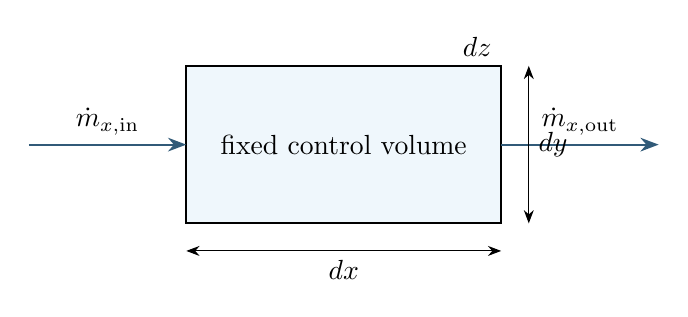
\begin{tikzpicture}[>=Stealth,scale=1]
\fill[softblue] (0,0) rectangle (4,2);
\draw[thick] (0,0) rectangle (4,2);
\draw[thick,->,deepblue] (-2,1) -- (0,1);
\draw[thick,->,deepblue] (4,1) -- (6,1);
\node[above] at (-1,1) {$\dot m_{x,\mathrm{in}}$};
\node[above] at (5,1) {$\dot m_{x,\mathrm{out}}$};
\node[align=center] at (2,1) {fixed control volume};
\draw[<->] (0,-.35)--node[below]{$dx$}(4,-.35);
\draw[<->] (4.35,0)--node[right]{$dy$}(4.35,2);
\node[above left] at (4,2) {$dz$};
\end{tikzpicture}
\caption{Differential control volume. The mass flux $\rho u$ varies slightly between the left and right faces.}
\end{figure}

If $\rho$ is smooth, the rate of mass accumulation in this small fixed volume is approximately
\[
\frac{\partial\rho}{\partial t}\,dx\,dy\,dz.
\]
The inlet and outlet mass flow rates in the $x$-direction are, to first order,
\[
\dot m_{x,\mathrm{in}}=(\rho u)\,dy\,dz,\qquad
\dot m_{x,\mathrm{out}}=\left[\rho u+\frac{\partial(\rho u)}{\partial x}\,dx\right]dy\,dz.
\]
Hence the net outward rate is
\[
\dot m_{x,\mathrm{out}}-\dot m_{x,\mathrm{in}}
=\frac{\partial(\rho u)}{\partial x}\,dx\,dy\,dz.
\]
Repeating this for the other four faces, adding accumulation, and dividing by $dx\,dy\,dz$ yields the pointwise equation.

\begin{proposition}[Differential continuity equation]
\[
\frac{\partial\rho}{\partial t}
+\frac{\partial(\rho u)}{\partial x}
+\frac{\partial(\rho v)}{\partial y}
+\frac{\partial(\rho w)}{\partial z}=0.
\]
Equivalently,
\[
\frac{\partial\rho}{\partial t}+\nabla\cdot(\rho\mathbf V)=0.
\]
No assumption of steady or incompressible flow is required.
\end{proposition}

\section{Incompressible Flow}

\begin{definition}[Incompressible flow]
An incompressible flow is one in which the volume of each material fluid parcel remains constant as it moves. Since a material parcel also conserves its mass, its density remains constant along the trajectory:
\[
\frac{D\rho}{Dt}=0.
\]
\end{definition}

Expanding the general continuity equation,
\[
\frac{\partial\rho}{\partial t}
+\mathbf V\cdot\nabla\rho+\rho\nabla\cdot\mathbf V=0,
\qquad\text{or}\qquad
\frac{D\rho}{Dt}+\rho\nabla\cdot\mathbf V=0.
\]
Thus, when $\rho>0$,

\begin{corollary}[Incompressible continuity equation]
\[
\nabla\cdot\mathbf V=0
\quad\Longleftrightarrow\quad
\frac{\partial u}{\partial x}+
\frac{\partial v}{\partial y}+
\frac{\partial w}{\partial z}=0.
\]
\end{corollary}

\textbf{Physical meaning.} Velocity divergence measures the instantaneous fractional rate at which a material parcel expands or contracts. Zero divergence means its volume is constant, even if its shape changes.

\begin{remark}
Incompressibility does not necessarily imply $\partial\rho/\partial t=0$. Density can change at a fixed point when different parcels pass through it. Assuming that $\rho$ is constant everywhere is a stronger condition.
\end{remark}

\section{Physics Olympiad Applications}

\begin{mathbox}
\textbf{Given: cylindrical coordinates}

For $\mathbf V=v_r\mathbf e_r+v_\theta\mathbf e_\theta+v_z\mathbf e_z$,
\[
\nabla\cdot\mathbf V=
\frac{1}{r}\frac{\partial(rv_r)}{\partial r}
+\frac{1}{r}\frac{\partial v_\theta}{\partial\theta}
+\frac{\partial v_z}{\partial z}.
\]
For an axisymmetric flow without swirl,
\[
\nabla\cdot\mathbf V=
\frac{1}{r}\frac{\partial(rv_r)}{\partial r}
+\frac{\partial v_z}{\partial z}.
\]
\end{mathbox}

\begin{problem}[Falling water jet, 2020 USAPhO B1, adapted]
Water falls steadily from a faucet with downward speed $v_0$ and jet radius $R_0$ at the spout. Use $(r,\theta,z)$ with $z$ positive upward. Let $R(z)$ be the radius of the stream and let $v(z)>0$ be the downward speed; the signed vertical velocity component is $v_z=-v(z)$.

Assume the water is incompressible, axisymmetric, and has no swirl. Neglect surface tension and take the dominant vertical speed to be independent of $r$; the radial component is small compared with the downward velocity. Use the result of part (a) without deriving it:
\[
v(z)=\sqrt{-2gz},\qquad z_0=-\frac{v_0^2}{2g},
\]
where $z=z_0$ at the faucet. Find $R(z)$ without initially assuming $Q=Av$.
\end{problem}

\begin{solution}
\begin{enumerate}
\item Since $v_z=-v(z)$ and the flow is steady,
\[
a_z=v_z\frac{\partial v_z}{\partial z}
=v\frac{dv}{dz}=-g.
\]
\item Continuity gives
\[
\frac1r\frac{\partial(rv_r)}{\partial r}=\frac{dv}{dz}.
\]
Integration in $r$, requiring finite $v_r$ at the axis, yields
\[
v_r(r,z)=\frac r2\frac{dv}{dz}.
\]
\item A surface particle satisfies $r-R(z)=0$ throughout its motion. Hence
\[
\frac D{Dt}[r-R(z)]=0
\quad\Longrightarrow\quad
v_r(R(z),z)=-v\frac{dR}{dz}.
\]
\item Equating the two boundary expressions gives
\[
\frac R2\frac{dv}{dz}=-v\frac{dR}{dz}
\quad\Longrightarrow\quad
\frac d{dz}(R^2v)=0.
\]
Using $R(z_0)=R_0$ and $v(z_0)=v_0$,
\[
\boxed{R(z)=R_0\sqrt{\frac{v_0}{v(z)}}=
R_0\left(\frac{v_0^2}{-2gz}\right)^{1/4}}.
\]
The jet narrows as the downward speed increases; the small radial velocity points inward.
\end{enumerate}
\end{solution}

\begin{problem}[Draining cylinder, 2018 INPhO Q7, adapted]
A water-filled cylinder of diameter $D$ is inverted into a basin of water. Air enters through a small hole of diameter $d$, causing the internal water level $h(t)$ to fall, with $h(0)=h_0>0$. Assume constant air and water densities, negligible losses, and $d\ll D$. A pressure and Bernoulli argument gives the air-entry speed
\[
v_a(h)=\sqrt{\frac{2\rho_wgh}{\rho_a}},
\]
where $\rho_w$ and $\rho_a$ denote the water and air densities.
\end{problem}

\begin{solution}
\begin{enumerate}
\item The incoming air volume rate equals the decrease in the water-filled volume:
\[
\frac{\pi d^2}{4}v_a=-\frac{\pi D^2}{4}\frac{dh}{dt}.
\]
\item Substituting the given $v_a(h)$ gives
\[
\frac{dh}{dt}=-K\sqrt h,\qquad
K=\frac{d^2}{D^2}\sqrt{\frac{2\rho_wg}{\rho_a}}.
\]
Separating variables and using $h(0)=h_0$,
\[
\boxed{h(t)=\left(\sqrt{h_0}-\frac{Kt}{2}\right)^2},
\qquad 0\le t\le t_{\mathrm{empty}}.
\]
\item The modeled emptying time is
\[
t_{\mathrm{empty}}=\frac{2\sqrt{h_0}}{K}.
\]
The flow is unsteady; both fluid densities are treated as constant in this approximation.
\end{enumerate}
\end{solution}
\end{document}
